\section{Workflows and Workflow Management Systems}

Workflows and workflow management systems are another tool to increase the flexibility of businesses in times of change, similar to SOA.
\citeauthor*{workflow:referencemodel} defines a workflow as "the computerised facilitation or automation of a business process, in whole or part"~\autocite{workflow:referencemodel}.
In other words, a workflow describes the tasks associated with a business process and the order in which these tasks are to be executed in such a way that they can be automated with the help of computers.
Workflows are often visually represented as directed graphs, with vertices representing the tasks and edges defining the order of these tasks.
\autoref{image:workflow} such a graph that represents a simple business workflow.
Note that the tasks can be a mixture of human and automated tasks.
In \autoref{image:workflow} for example, the identify payment method, accept cash, and prepare package tasks could be executed by humans, while the process credit card task would be handled by a computer program.
Moreover, in combination with SOA, the process credit card task could be a call to an external service provided by an PCI\footnote{\nom{Payment Card Industry}{PCI}: The PCI Security Standards Council developed a data security standard (PCI DSS)\footnotemark to enhance the security of credit card information. Businesses handling credit card information are encouraged to comply with these requirements to prevent security breaches and improve trust. Since this can be a complicated process, outsourcing credit card handling can save time and effort.} compliant business specialized in payment processing.

\footnotetext{{\url{https://www.pcisecuritystandards.org/documents/PCI_DSS_v3.pdf}}}

\begin{figure}[!htbp]
	\centering
	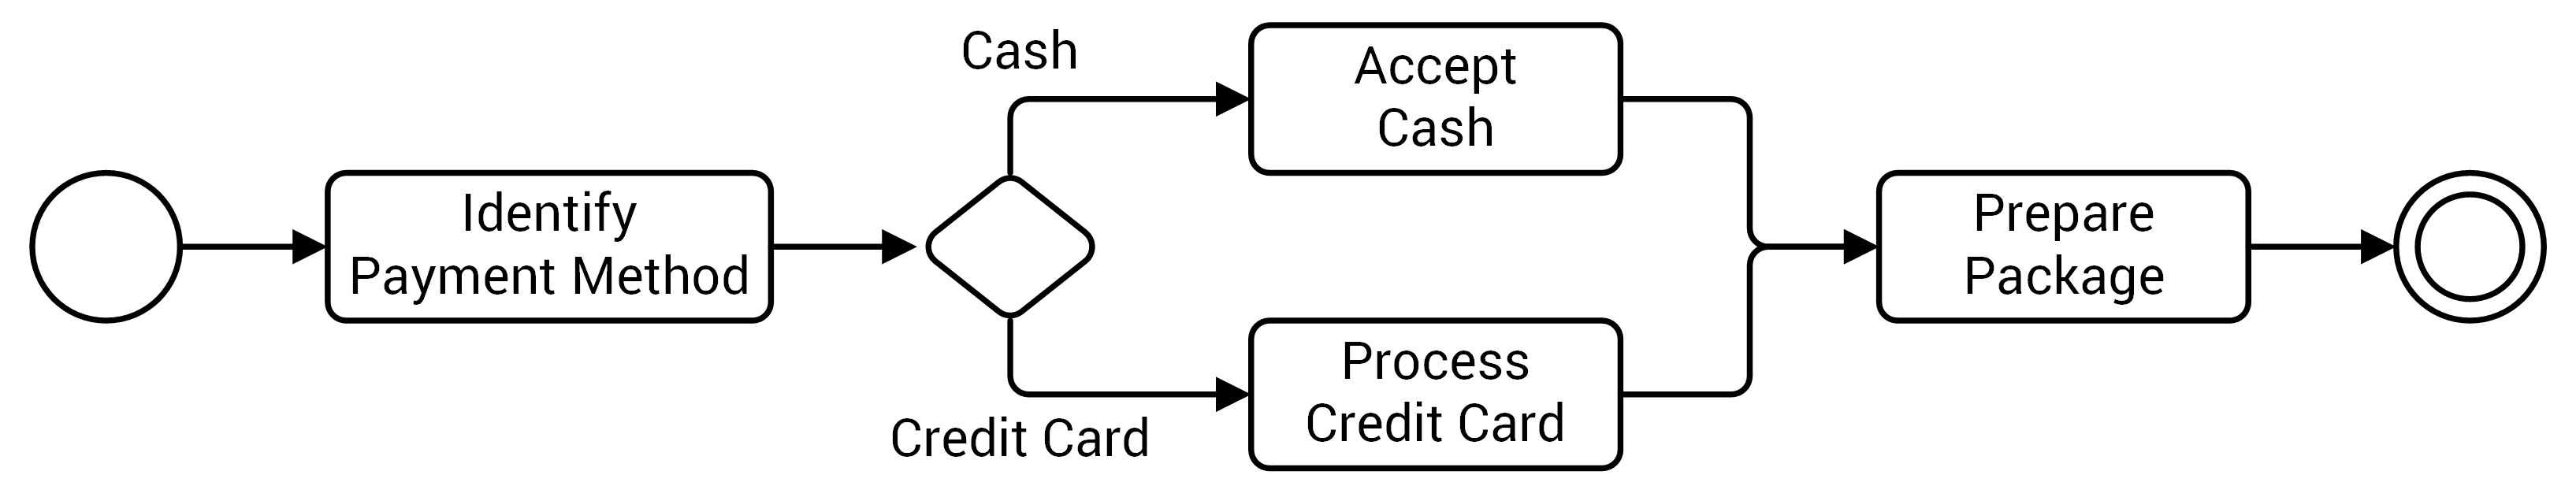
\includegraphics[resolution=600]{fundamentals/assets/workflow}
	\caption{A simple workflow represented as a graph.}
	\label{image:workflow}
\end{figure}

The automation of a workflow is handled by a workflow management system, which \citeauthor*{workflow:referencemodel} defines as "a system that completely defines, manages and executes workflows through the execution of software whose order of execution is driven by a computer representation of the workflow logic"~\autocite{workflow:referencemodel}.
In other words, a workflow management system receives a workflow as input and then executes the actions associated with each workflow task in the particular order described by the workflow.
For the example in \autoref{image:workflow}, this could mean that the workflow management system presents an employee with a graphical user interface, where they can select the payment method based on the choice of a customer.
If the customer chooses to pay cash, the workflow management system would then show a dialog where the employee could enter this cash transaction.
If the customer chooses to pay with a credit card, the workflow management system would call an external service with the credit card details to approve the transaction.
In the final step, the workflow management system could assist the employee with preparing the package by automatically printing a label or displaying useful information.

In the past, workflows have been mainly applied in a business context, in particular for modeling and re-engineering of business processes.
This lead to the development of business-centered standards like BPEL or BPMN to describe workflows, and corresponding workflow management system that can execute these workflows.
One particular characteristic of these business workflows is that they are fairly static, i.e. they will not change during a workflow execution and only rarely in between due to business process re-engineering.
This also means that the existing business workflow infrastructure is geared towards these static workflows~\autocite{wasa}.

In recent years however, new applications for the use of workflows have emerged, among them scientific workflows.
These scientific workflows differ from business workflows in that they are much more dynamic and therefore require more flexibility in the tools supporting them.
The reason for this is that the processes involved in scientific workflows are rarely completely know in advance.
Exploration and trial and error often play a role, which can lead to unpredictable changes in the processes~\autocite{wasa}.
Existing workflow technology often can't offer the required flexibility for scientific workflows, which is why modification of existing technology or creation of new technology is required to fully support scientific workflows.
Therefore, \nom{scientific workflow management systems}{SWfMSs} have been created, which offer scientist adequate support throughout the experimentation process.
